\documentclass{beamer}
\mode<presentation>
\usetheme{default}
\usecolortheme{default}


\usepackage{color}
\usepackage{graphicx}
\usepackage{pgffor}
\usepackage{epigraph}

\title[Doctorate] %optional
{What Exactly Is a Doctorate?}

\author[Matt Might]
{Matt Might}

\begin{document}
\titlepage

\begin{frame}
	Every fall, I\footnote{Matt Might is a professor of Computer Science at the University of Utah. He tweets from @mattmight and blogs at blog.might.net.} explain to a fresh batch of Ph.D. students what a Ph.D. is. It's hard to describe it in words. So, I use pictures. Read below for the illustrated guide to a Ph.D.
\end{frame}

\begin{frame}
	Imagine a circle that contains all of human knowledge:
	\center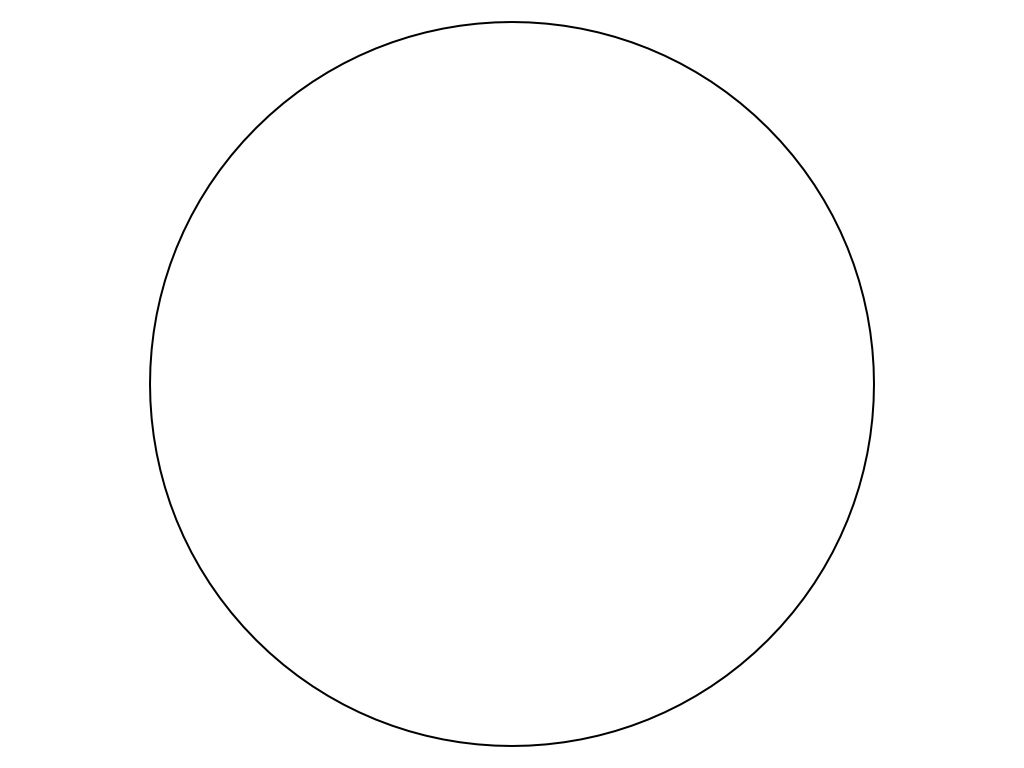
\includegraphics[width=0.9\textwidth]{figures/fig_1}
\end{frame}

\begin{frame}
	By the time you finish elementary school, you know a little:
	\center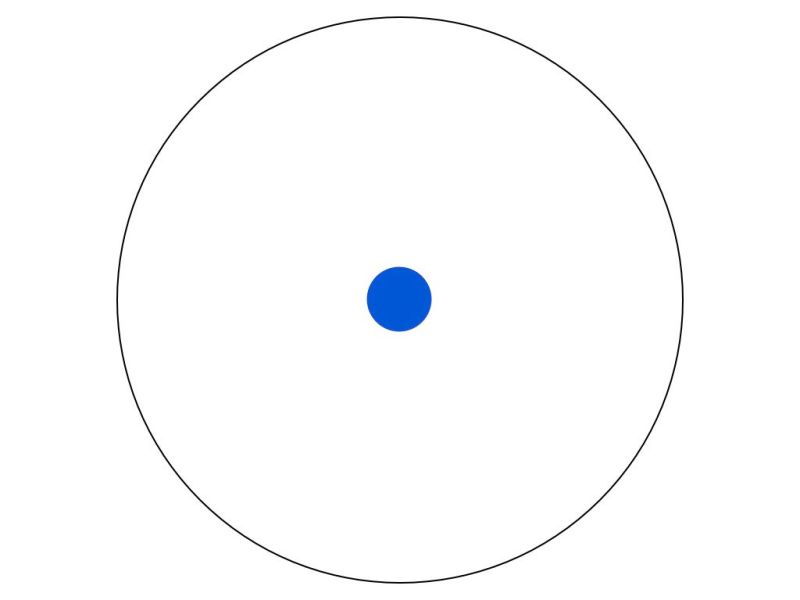
\includegraphics[width=0.9\textwidth]{figures/fig_2}
\end{frame}

\begin{frame}
	By the time you finish high school, you know a bit more:
	\center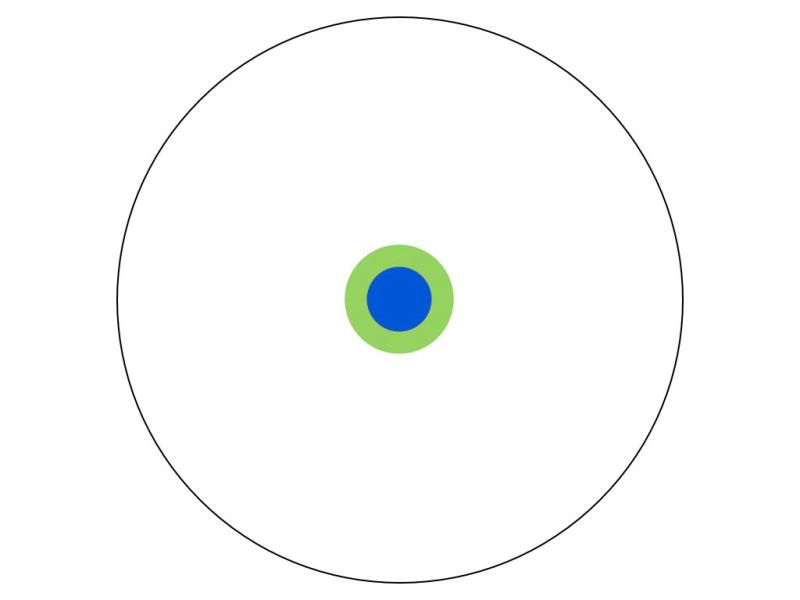
\includegraphics[width=0.9\textwidth]{figures/fig_3}
\end{frame}

\begin{frame}
	With a bachelor's degree, you gain a specialty:
	\center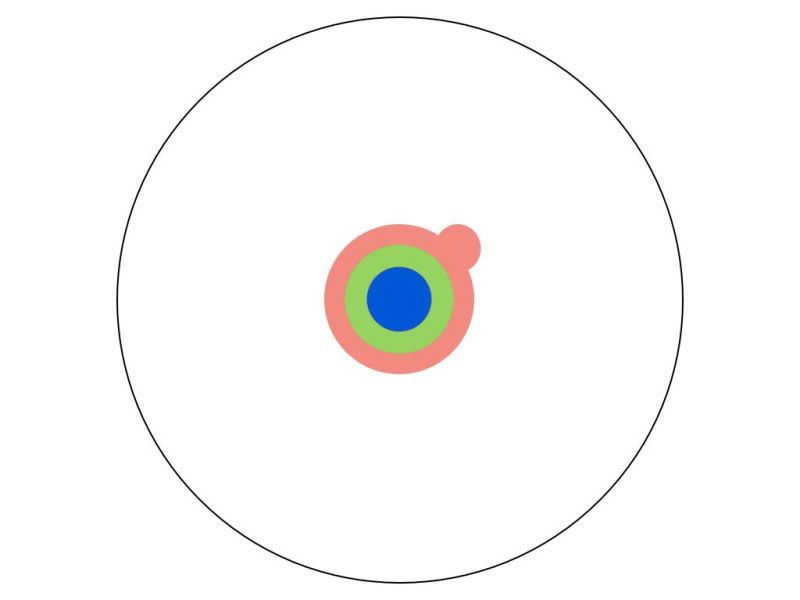
\includegraphics[width=0.9\textwidth]{figures/fig_4}
\end{frame}

\begin{frame}
	A master's degree deepens that specialty:
	\center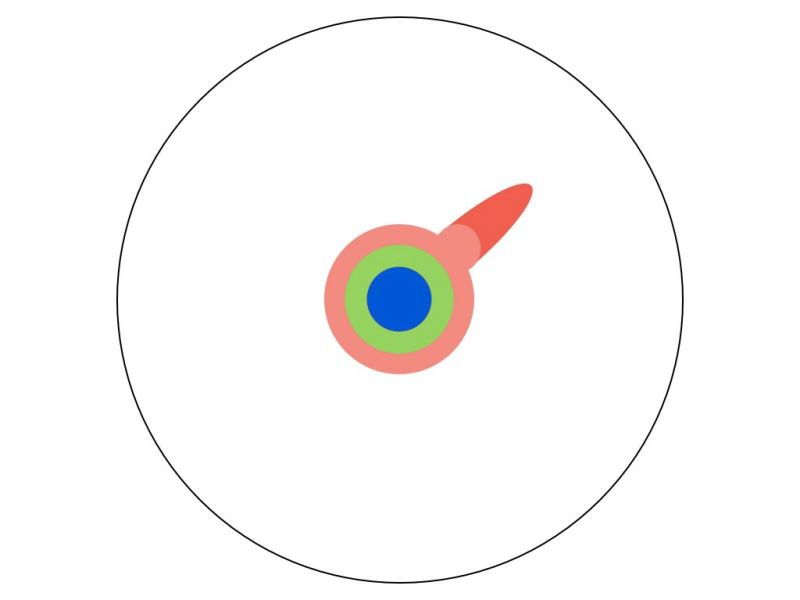
\includegraphics[width=0.9\textwidth]{figures/fig_5}
\end{frame}

\begin{frame}
	Reading research papers takes you to the edge of human knowledge:
	\center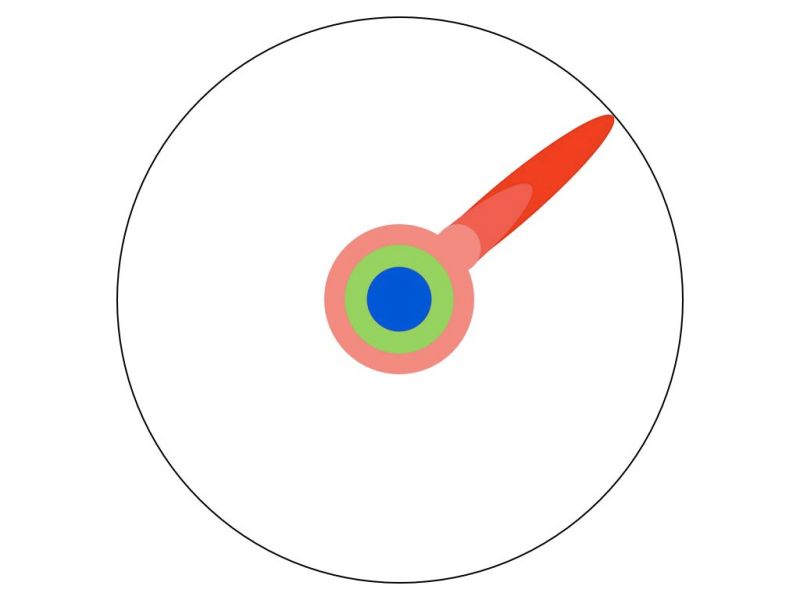
\includegraphics[width=0.9\textwidth]{figures/fig_6}
\end{frame}

\begin{frame}
	Once you're at the boundary, you focus:
	\center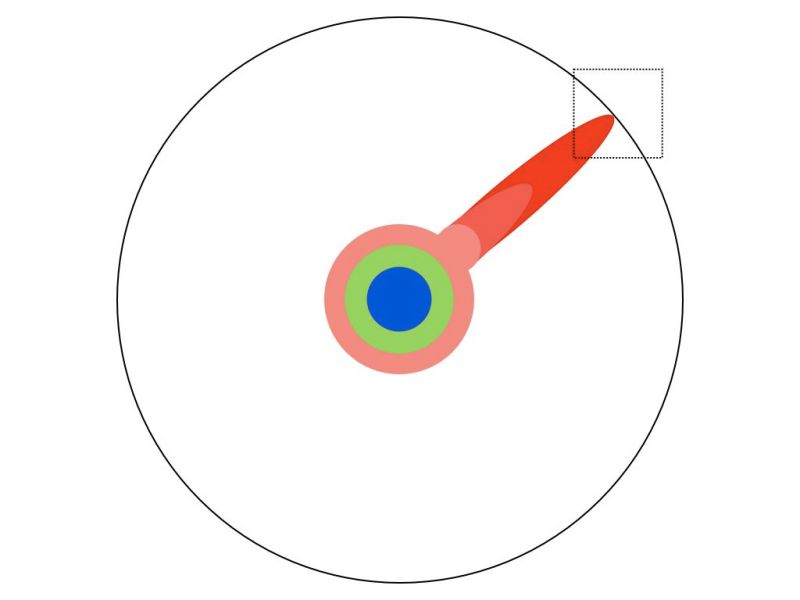
\includegraphics[width=0.9\textwidth]{figures/fig_7}
\end{frame}

\begin{frame}
	You push at the boundary for a few years:
	\center
\includegraphics[width=0.9\textwidth]{figures/fig_8}
\end{frame}

\begin{frame}
	Until one day, the boundary gives way:
	\center
\includegraphics[width=0.9\textwidth]{figures/fig_9}
\end{frame}

\begin{frame}
	And, that dent you've made is called a Ph.D.:
	\center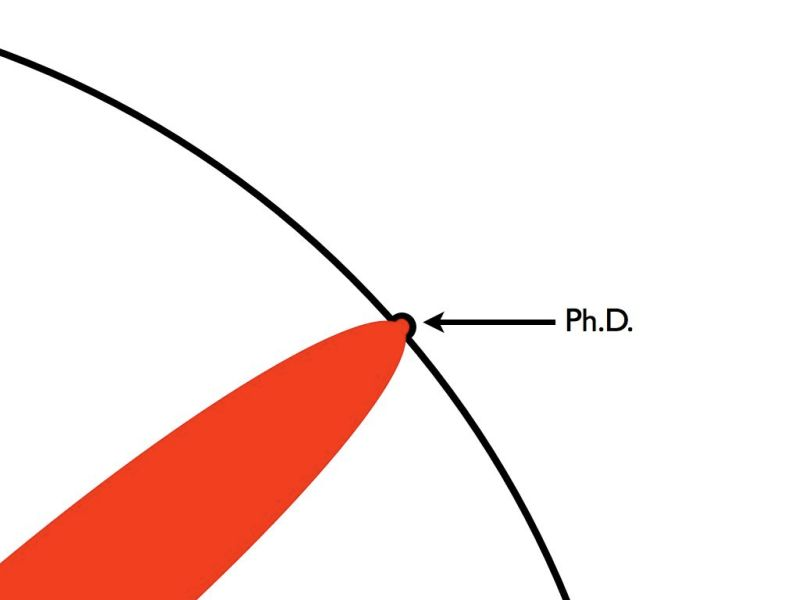
\includegraphics[width=0.9\textwidth]{figures/fig_10}
\end{frame}

\begin{frame}
	Of course, the world looks different to you now:
	\center
\includegraphics[width=0.9\textwidth]{figures/fig_11}
\end{frame}

\begin{frame}
	So, don't forget the bigger picture:
	\center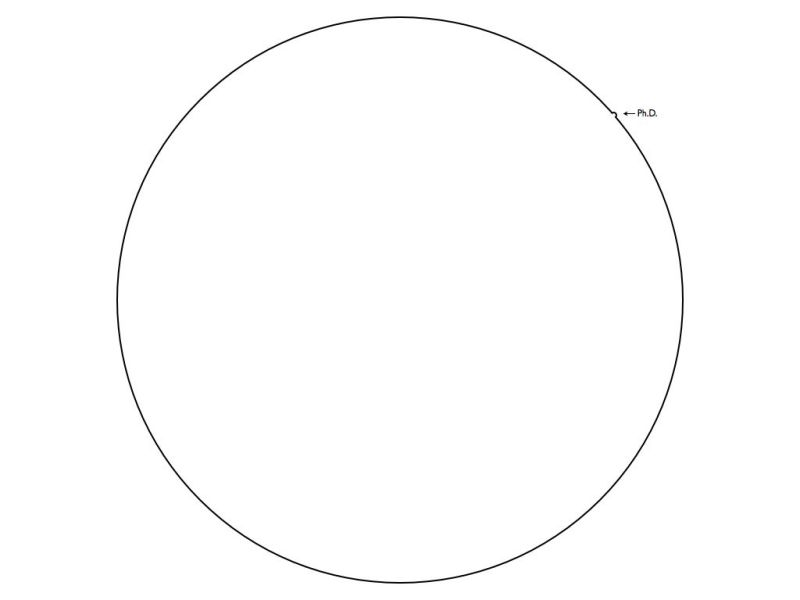
\includegraphics[width=0.9\textwidth]{figures/fig_12}
\end{frame}

\begin{frame}
	\huge{Keep pushing.}
	
	\vfill
	
\end{frame}
\end{document}
